\section{传输线理论}

凡是能够导引电磁波沿一定方向传输的导体、介质系统均可称为传输线。微波传输线不仅可以用来传输电磁能量,还可用来构成各种微波元件。微波传输线种类繁多,按其传输的电磁波波型,大致可划分为三种类型。

\subsection{微波的传播特性}

与射频一样,微波是非电离且非破坏性的,从本质上来说,对人类是安全的。微波是一种高频电磁波,其波长范围为 0.3 mm 至 300 mm(对应频率范围为 1 GHz 至 1 THz)。由于其波长较长,微波的穿透能力比可见光、紫外线或 X射线强,但比低频无线电波弱。微波无线电P传播的路径损耗(Lp)是无线通信和成像的一个主要参数,由Friis公式\cite{huang2021antennas}控制

\begin{equation}
	L_{\mathrm{p}} = 10 \times \lg \left( \frac{P^{\mathrm{t}}}{P^{\mathrm{r}}} \right) = 20 \times \lg f + 20 \times \lg r - 147.6 \ (\text{in dB})
	\tag{1}
\end{equation}



其中,Pt是发射器功率;Pr是接收器功率;f是频率;r是距离。我们可以看出,路径损耗与频率f的平方和距离r的平方成正
比。频率越高,路径损耗就越大。


\subsection{传输线及其方程的解}

传输线方程是研究传输线上电压、电流的变化规律及其相互关系的方程。它可由均匀传输线的等效电路导出。

\begin{figure}[htbp]
	\centering
	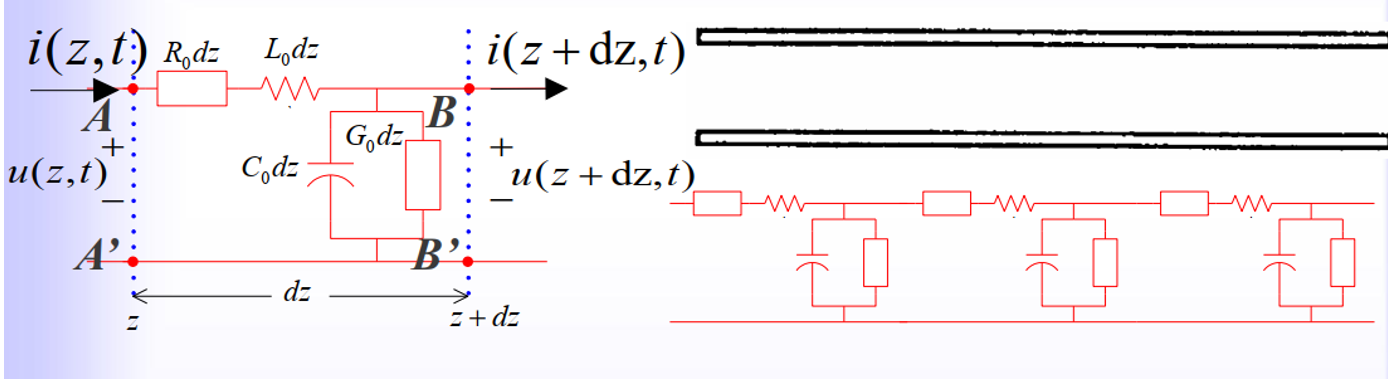
\includegraphics[width=0.8\linewidth]{img/2-1.png}
	\caption{传输线等效电路图}
	\label{fig:2-1}
\end{figure}

对于均匀传输线,取一个微元段 \( \mathrm{d}z \),其集中参数分别为 \( R_0 \, \mathrm{d}z \)、\( G_0 \, \mathrm{d}z \)、\( L_0 \, \mathrm{d}z \) 及 \( C_0 \, \mathrm{d}z \)。

等效电路如图 2 所示。传输线的始端接角频率为 ω 的正弦信号源,终端接负载阻抗 Z 
L。坐标原点选在始端。设距始端 z 处的电压和电流分别为 u 和 i,经过 dz 段后电压和电流分别为 u−du 和 i−di。传输线上的电压 u 和电流 i 既是位置坐标 z 的函数又是时间 t 的函数,可分别表示为 u=u(z,t),i=i(z,t)。经过 dz 段后电压和电流的变化量为


\begin{equation}
	\begin{cases}
		\displaystyle \frac{u(z + \mathrm{d}z, t) - u(z, t)}{\mathrm{d}z} = -R_0 \cdot i(z, t) - L_0 \cdot \frac{\partial i(z, t)}{\partial t} \\[12pt]
		\displaystyle \frac{i(z + \mathrm{d}z, t) - i(z, t)}{\mathrm{d}z} = -G_0 \cdot u(z + \mathrm{d}z, t) - C_0 \cdot \frac{\partial u(z + \mathrm{d}z, t)}{\partial t}
	\end{cases}
	\tag{2}
\end{equation}


\begin{equation}
	\begin{aligned}
		& \left\{
		\begin{aligned}
			\frac{\partial u(z, t)}{\partial z} &= -R_0 \cdot i(z, t) - L_0 \cdot \frac{\partial i(z, t)}{\partial t} \\
			\frac{\partial i(z, t)}{\partial z} &= -G_0 \cdot u(z, t) - C_0 \cdot \frac{\partial u(z, t)}{\partial t}
		\end{aligned}
		\right. \\
		& \quad \text{\tikzmarknode{eq1}{}} \quad \text{\tikzmarknode{eq2}{}} \\
		& \left\{
		\begin{aligned}
			\frac{d^2 U(z)}{dz^2} - \gamma^2 U(z) &= 0 \\
			\frac{d^2 I(z)}{dz^2} - \gamma^2 I(z) &= 0
		\end{aligned}
		\right.
	\end{aligned}
	\tag{2-2-3}
\end{equation}

如上公式2-2-3所示,1为时域电报方程,2为频域电报方程。时域电报方程描述了传输线上电压 u(z,t) 和电流 i(z,t) 随位置 z 和时间 t 的变化规律。频域电报方程是时域电报方程的傅里叶变换形式,主要用于分析稳态正弦信号在传输线上的传播特性。

\begin{equation}
	\begin{aligned}
		& \left\{
		\begin{aligned}
			U(z) &= A_1 e^{-\gamma z} + A_2 e^{\gamma z} \\
			I(z) &= \frac{1}{Z_0} \big( A_1 e^{-\gamma z} - A_2 e^{\gamma z} \big)
		\end{aligned}
		\right. \\
		& \quad \text{\tikzmarknode{eq3}{}} \quad \text{\tikzmarknode{eq4}{}} \\
		& \left\{
		\begin{aligned}
			U(z) &= U_i(z) + U_r(z) = U_i(z) [1 + \Gamma(z)] \\
			I(z) &= I_i(z) + I_r(z) = I_i(z) [1 - \Gamma(z)]
		\end{aligned}
		\right.
	\end{aligned}
	\tag{2-2-4}
\end{equation}

这两个公式分别描述了传输线上的电压和电流分布,以及入射波与反射波的关系。公式1这组公式描述了传输线上电压 U(z) 和电流 I(z) 的分布。
z 表示沿传输线的位置坐标,从参考点(通常为传输线的始端)开始测量。
公式2这组公式描述了传输线上的总电压和总电流如何由入射波和反射波组成。
$U(z)$ 和 $I(z)$ 分别是总电压和总电流,而 $U_i(z)$、$U_r(z)$、$I_i(z)$、$I_r(z)$ 分别表示入射波和反射波的电压和电流分量。



\subsection{传输线的特性参量}
传输线的特性参数主要包括:传播常数、特性阻抗、相速和相波长、输入阻抗、反射系数、驻波比(行波系数)和传输功率等。下面以相对重要的传播参数和特性阻抗分别加以介绍。

\subsubsection{传播参数}

\[
\gamma = \sqrt{(R_0 + j \omega L_0)(G_0 + j \omega C_0)} = \alpha + j \beta
\]

- $\alpha$ 是衰减常数,表示行波每经过单位长度后振幅的衰减倍数,其单位为分贝/米 (dB/m) 或奈培/米 (Np/m);
- $\beta$ 是相位常数,表示行波每经过单位长度后相位滞后的弧度数,单位为弧度/米 (rad/m)。

\[
\gamma = j \omega \sqrt{L_0 C_0} = j \beta \quad (\beta = \omega \sqrt{L_0 C_0})
\]

\subsubsection{特性阻抗}

\[
Z_0 = \frac{U_i}{I_i} = -\frac{U_r}{I_r} \quad (\text{定义})
\]
\[
Z_0 = \sqrt{\frac{Z}{Y}} = \sqrt{\frac{R_0 + j \omega L_0}{G_0 + j \omega C_0}}
\]
\[
Z_0 = \sqrt{\frac{L_0}{C_0}} \quad (\text{无耗传输线})
\]

\subsubsection{相位关系与波速}

\[
\text{Pha.} = \omega t - \beta z = \text{Constant}
\]
两边求导:
\[
v_p = \frac{dz}{dt} = \frac{\omega}{\beta} \quad (\text{时域解})
\]

上式均适用有耗/无耗传输线。

\subsubsection{波长与频率的关系}

\[
\lambda_p = \frac{v_p}{f} = \frac{2\pi}{\beta}
\]


\subsection{阻抗圆图及应用}
在微波工程中,经常会遇到输入阻抗、负载阻抗、反射系数和驻波比等参数的计算问题;此外,还有阻抗匹配方面的问题。若用前面介绍的公式计算,会遇到大量的复数运算,非常繁琐。工程上常用阻抗圆图来分析和计算,既方便又直观,而且具有一定精度,可满足工程设计要求,因而圆图作为处理微波传输线问题的一种图解法,在实际中获得了普遍应用。

下面介绍圆图的构造、原理及其应用。为了使阻抗圆图适用于任意特性阻抗的传输线的计算,故圆图上的阻抗均采用归一化阻抗。

\begin{figure}[htbp]
	\centering
	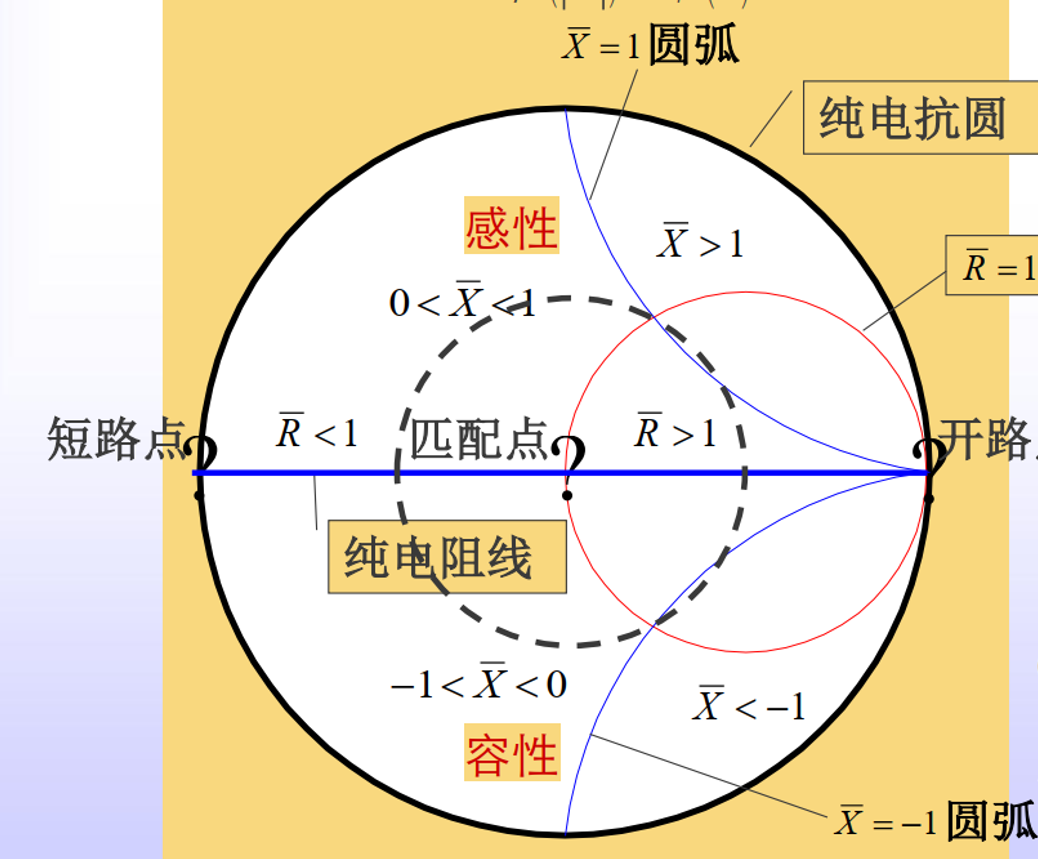
\includegraphics[width=0.5\linewidth]{img/2-4}
	\caption{阻抗圆图及其重要的点线面}
	\label{fig:2-4}
\end{figure}

(1) 三个圆族:反射系数圆;等电阻圆;等电抗圆。

(2) 三个特殊点:
开路点;匹配点;短路点。

(3) 三条特殊线:
纯电阻线;纯电抗圆;可匹配圆(串联)。

(4) 二个特殊面:
上半圆平面(感性)和下半圆平面(容性)。

(5) 二个旋转方向:
“源顺负逆”。
